\documentclass{beamer}

\usepackage{tikz}
\usetikzlibrary{patterns}
\usetikzlibrary{calc}
\usetikzlibrary{shapes, arrows, positioning}

\usepackage{tabularray}
\UseTblrLibrary{booktabs}
\DefTblrTemplate{contfoot-text}{normal}{\lang{(Continued on next page)}{(Continua na próxima página)}} 
\SetTblrTemplate{contfoot-text}{normal} 
\DefTblrTemplate{conthead-text}{normal}{\lang{(continued)}{(continuação)}} 
\SetTblrTemplate{conthead-text}{normal}

\usepackage{enumitem}
\definecolor{ifscgreen}{RGB}{50,93,61}

\setlist[enumerate,1]{label=\colorbox{ifscgreen}{\textcolor{white}{\arabic*}}\quad, leftmargin=*}
\setlist[enumerate,2]{label=\colorbox{ifscgreen!70}{\textcolor{white}{\arabic{enumi}.\arabic*}}\quad, leftmargin=*}
\setlist[enumerate,3]{label=\colorbox{ifscgreen!40}{\textcolor{white}{\arabic{enumi}.\arabic{enumii}.\arabic*}}\quad, leftmargin=*}
% ------------------------------
% Codificação e idioma
% ------------------------------
% \usepackage[utf8]{inputenc}
\usepackage[T1]{fontenc}
\usepackage[brazil]{babel}

% ------------------------------
% Matemática e símbolos
% ------------------------------
\usepackage{amsmath}

% ------------------------------
% Gráficos e figuras
% ------------------------------
\usepackage{graphicx}
\usepackage{subfigure}

% ------------------------------
% Cores, URL e hiperlinks
% ------------------------------
\usepackage{url,color}
\usepackage{hyperref}
\hypersetup{
  pdfstartview={Fit},
  pdftitle={\@title},
  pdfsubject={Engenharia de Telecomunicacoes - IFSC},
  pdfauthor={\@author}
}

% ------------------------------
% Listagens e pseudocódigo
% ------------------------------
\usepackage[
plainruled,
noline
]{algorithm2e}

% ------------------------------
% Bibliografia
% ------------------------------
\usepackage[backend=biber,style=numeric,citestyle=ieee]{biblatex}
\addbibresource{../../latex/references.bib}
\setbeamertemplate{bibliography item}{\insertbiblabel}

% ------------------------------
% Outros pacotes
% ------------------------------
\usepackage{../../latex/ifsc_slides} % (pacote personalizado, ok manter)

% ------------------------------
% Macros e comandos personalizados
% ------------------------------
\newcommand{\tab}[1]{\hspace{.2\textwidth}\rlap{#1}}

\newcommand{\DAY}{\the\day}
\newcommand{\MONTH}{%
  \ifcase\the\month
  \or Janeiro%
  \or Fevereiro%
  \or Março%
  \or Abril%
  \or Maio%
  \or Junho%
  \or Julho%
  \or Agosto%
  \or Setembro%
  \or Outubro%
  \or Novembro%
  \or Dezembro%
  \fi}
\newcommand{\YEAR}{\the\year}

% ------------------------------
% Dados do título
% ------------------------------
\title{EMB22109 - Sistemas Embarcados:}
\subtitle{\LARGE Introdução a SOs e Tipos de Kernel}
\author{João Cláudio Elsen Barcellos}
\date{\scriptsize \DAY~de \MONTH~de \YEAR}
\institute{
  Engenheiro Eletricista\\
  Formado na Universidade Federal de Santa Catarina\\
  campus Florianópolis\\
  \url{joaoclaudiobarcellos@gmail.com}
}

% ------------------------------
% Customização das seções no Beamer
% ------------------------------
\def\sectionname{}
\def\insertsectionnumber{}
\def\subsectionname{}
\def\insertsubsectionnumber{}

\AtBeginSection[]{
  \begin{frame}
      \vfill
      \centering
      \begin{beamercolorbox}[sep=8pt,center,shadow=true,rounded=true]{title}
          \usebeamerfont{title}\insertsectionhead\par%
      \end{beamercolorbox}
      \vfill
  \end{frame}
}

\setbeamertemplate{caption}[numbered]

% ------------------------------
% Controle de idioma
% ------------------------------
\usepackage{ifthen}
\newboolean{english}
\setboolean{english}{false} % true = inglês, false = português

% Configuração de idioma e títulos
\ifthenelse{\boolean{english}}{
  \usepackage[english]{babel}
  \renewcommand{\figurename}{Figure}
  \renewcommand{\tablename}{Table}
  \SetAlgorithmName{Algorithm}{}{}
  
  \SetKwInput{KwData}{Input}
  \SetKwInput{KwResult}{Output}
  \SetKwIF{If}{ElseIf}{Else}{if}{then}{else if}{else}{end if}
  \SetKwFor{While}{while}{do}{end while}
  \SetKwFor{For}{for}{do}{end for}
  \SetKw{Return}{return}
}{
  \usepackage[brazil]{babel}
  \renewcommand{\figurename}{Figura}
  \renewcommand{\tablename}{Tabela}
  \SetAlgorithmName{Algoritmo}{}{}
  
  \SetKwInput{KwData}{Entrada}
  \SetKwInput{KwResult}{Saída}
  \SetKwIF{If}{ElseIf}{Else}{se}{então}{senão se}{senão}{fim}
  \SetKwFor{While}{enquanto}{faça}{fim}
  \SetKwFor{For}{para}{faça}{fim}
  \SetKw{Return}{retorna}
}
% Comando para alternar entre idiomas (inglês/português)
\newcommand{\lang}[2]{\ifbool{english}{#1}{#2}}
    
% Default fixed font does not support bold face
\DeclareFixedFont{\ttb}{T1}{txtt}{bx}{n}{8} % for bold
\DeclareFixedFont{\ttm}{T1}{txtt}{m}{n}{8}  % for normal

% Custom colors
\usepackage{color}
\definecolor{deepblue}{rgb}{0,0,0.5}
\definecolor{deepred}{rgb}{0.6,0,0}
\definecolor{deepgreen}{rgb}{0,0.5,0}

\usepackage{listings}

% Python style for highlighting
\newcommand\pythonstyle{\lstset{
language=Python,
basicstyle=\ttm\tiny,
morekeywords={self},              % Add keywords here
keywordstyle=\ttb\color{deepblue},
emph={MyClass,__init__},          % Custom highlighting
emphstyle=\ttb\color{deepred},    % Custom highlighting style
stringstyle=\color{deepgreen},
frame=tb,                         % Any extra options here
showstringspaces=false,
numbers=none 
}}


% Python environment
\lstnewenvironment{python}[1][]
{
\pythonstyle
\lstset{#1}
}
{}

% Python for external files
\newcommand\pythonexternal[2][]{{
\pythonstyle
\lstinputlisting[#1]{#2}}}

% Python for inline
\newcommand\pythoninline[1]{{\pythonstyle\lstinline!#1!}}    
    
    \lstset{
      inputencoding = utf8,  % Input encoding
      extendedchars = true,  % Extended ASCII
      literate      =        % Support additional characters
      {á}{{\'a}}1  {é}{{\'e}}1  {í}{{\'i}}1 {ó}{{\'o}}1  {ú}{{\'u}}1
      {Á}{{\'A}}1  {É}{{\'E}}1  {Í}{{\'I}}1 {Ó}{{\'O}}1  {Ú}{{\'U}}1
      {à}{{\`a}}1  {è}{{\`e}}1  {ì}{{\`i}}1 {ò}{{\`o}}1  {ù}{{\`u}}1
      {À}{{\`A}}1  {È}{{\`E}}1  {Ì}{{\`I}}1 {Ò}{{\`O}}1  {Ù}{{\`U}}1
      {ä}{{\"a}}1  {ë}{{\"e}}1  {ï}{{\"i}}1 {ö}{{\"o}}1  {ü}{{\"u}}1
      {Ä}{{\"A}}1  {Ë}{{\"E}}1  {Ï}{{\"I}}1 {Ö}{{\"O}}1  {Ü}{{\"U}}1
      {â}{{\^a}}1  {ê}{{\^e}}1  {î}{{\^i}}1 {ô}{{\^o}}1  {û}{{\^u}}1
      {Â}{{\^A}}1  {Ê}{{\^E}}1  {Î}{{\^I}}1 {Ô}{{\^O}}1  {Û}{{\^U}}1
      {œ}{{\oe}}1  {Œ}{{\OE}}1  {æ}{{\ae}}1 {Æ}{{\AE}}1  {ß}{{\ss}}1
      {ẞ}{{\SS}}1  {ç}{{\c{c}}}1 {Ç}{{\c{C}}}1 {ø}{{\o}}1  {Ø}{{\O}}1
      {å}{{\aa}}1  {Å}{{\AA}}1  {ã}{{\~a}}1  {õ}{{\~o}}1 {Ã}{{\~A}}1
      {Õ}{{\~O}}1  {ñ}{{\~n}}1  {Ñ}{{\~N}}1  {¿}{{?`}}1  {¡}{{!`}}1
      {„}{\quotedblbase}1 {"}{\textquotedblleft}1 {–}{$-$}1
      {°}{{\textdegree}}1 {º}{{\textordmasculine}}1 {ª}{{\textordfeminine}}1
      {£}{{\pounds}}1  {©}{{\copyright}}1  {®}{{\textregistered}}1
      {«}{{\guillemotleft}}1  {»}{{\guillemotright}}1  {Ð}{{\DH}}1  {ð}{{\dh}}1
      {Ý}{{\'Y}}1    {ý}{{\'y}}1    {Þ}{{\TH}}1    {þ}{{\th}}1    {Ă}{{\u{A}}}1
      {ă}{{\u{a}}}1  {Ą}{{\k{A}}}1  {ą}{{\k{a}}}1  {Ć}{{\'C}}1    {ć}{{\'c}}1
      {Č}{{\v{C}}}1  {č}{{\v{c}}}1  {Ď}{{\v{D}}}1  {ď}{{\v{d}}}1  {Đ}{{\DJ}}1
      {đ}{{\dj}}1    {Ė}{{\.{E}}}1  {ė}{{\.{e}}}1  {Ę}{{\k{E}}}1  {ę}{{\k{e}}}1
      {Ě}{{\v{E}}}1  {ě}{{\v{e}}}1  {Ğ}{{\u{G}}}1  {ğ}{{\u{g}}}1  {Ĩ}{{\~I}}1
      {ĩ}{{\~\i}}1   {Į}{{\k{I}}}1  {į}{{\k{i}}}1  {İ}{{\.{I}}}1  {ı}{{\i}}1
      {Ĺ}{{\'L}}1    {ĺ}{{\'l}}1    {Ľ}{{\v{L}}}1  {ľ}{{\v{l}}}1  {Ł}{{\L{}}}1
      {ł}{{\l{}}}1   {Ń}{{\'N}}1    {ń}{{\'n}}1    {Ň}{{\v{N}}}1  {ň}{{\v{n}}}1
      {Ő}{{\H{O}}}1  {ő}{{\H{o}}}1  {Ŕ}{{\'{R}}}1  {ŕ}{{\'{r}}}1  {Ř}{{\v{R}}}1
      {ř}{{\v{r}}}1  {Ś}{{\'S}}1    {ś}{{\'s}}1    {Ş}{{\c{S}}}1  {ş}{{\c{s}}}1
      {Š}{{\v{S}}}1  {š}{{\v{s}}}1  {Ť}{{\v{T}}}1  {ť}{{\v{t}}}1  {Ũ}{{\~U}}1
      {ũ}{{\~u}}1    {Ū}{{\={U}}}1  {ū}{{\={u}}}1  {Ů}{{\r{U}}}1  {ů}{{\r{u}}}1
      {Ű}{{\H{U}}}1  {ű}{{\H{u}}}1  {Ų}{{\k{U}}}1  {ų}{{\k{u}}}1  {Ź}{{\'Z}}1
      {ź}{{\'z}}1    {Ż}{{\.Z}}1    {ż}{{\.z}}1    {Ž}{{\v{Z}}}1  {ž}{{\v{z}}}1
      % ¿ and ¡ are not correctly displayed if inconsolata font is used
      % together with the lstlisting environment. Consider typing code in
      % external files and using \lstinputlisting to display them instead.      
    }
    
\begin{document}

\captionsetup{labelformat=empty}

\begin{frame}[t]
    % \note{Boa tarde a todos, na aula de hoje iremos estudar os circuitos sequenciais...}
    \maketitle
    \vspace{-1cm}
    \begin{flushleft}
        \vfill
        \textit{\tiny $^{*}$Créditos ao Prof. Emerson Ribeiro de Mello, o qual criou e disponibilizou o template aqui usado, via ShareLaTeX}\par
        \textit{\tiny $^{**}$Créditos ao Prof. Hugo Marcondes, o qual forneceu parte do conteúdo usado nesta apresentação}
    \end{flushleft}
\end{frame}

\begin{frame}[t]{Na aula de hoje veremos...}
    \tableofcontents
\end{frame}

\section{Sistemas Embarcados}

\begin{frame}[fragile]
\frametitle{Revisão: Sistemas embarcados}

\begin{columns}
    \begin{column}{0.6\textwidth}
        \begin{enumerate}\footnotesize
            \item São sistemas computacionais desenvolvidos para realizar funções específicas;
            \item Usualmente constituem ``sistemas maiores'';
            \item Usualmente possuem diversas restrições e limitações (e.g., quantidade de memória, capacidade de processamento, gerenciamento de energia);
            \item Por vezes, usados em aplicações de \textit{real-time} e de alta confiabilidade (e.g., aplicações automotivas, aeroespaciais);
            \item Usualmente têm interação direta com o ambiente físico.
        \end{enumerate}
    \end{column}
    
    \begin{column}{0.4\textwidth}
        \begin{center}
            % https://magazine.raspberrypi.com/articles/cubesat-dual-redundant-flight-computer
            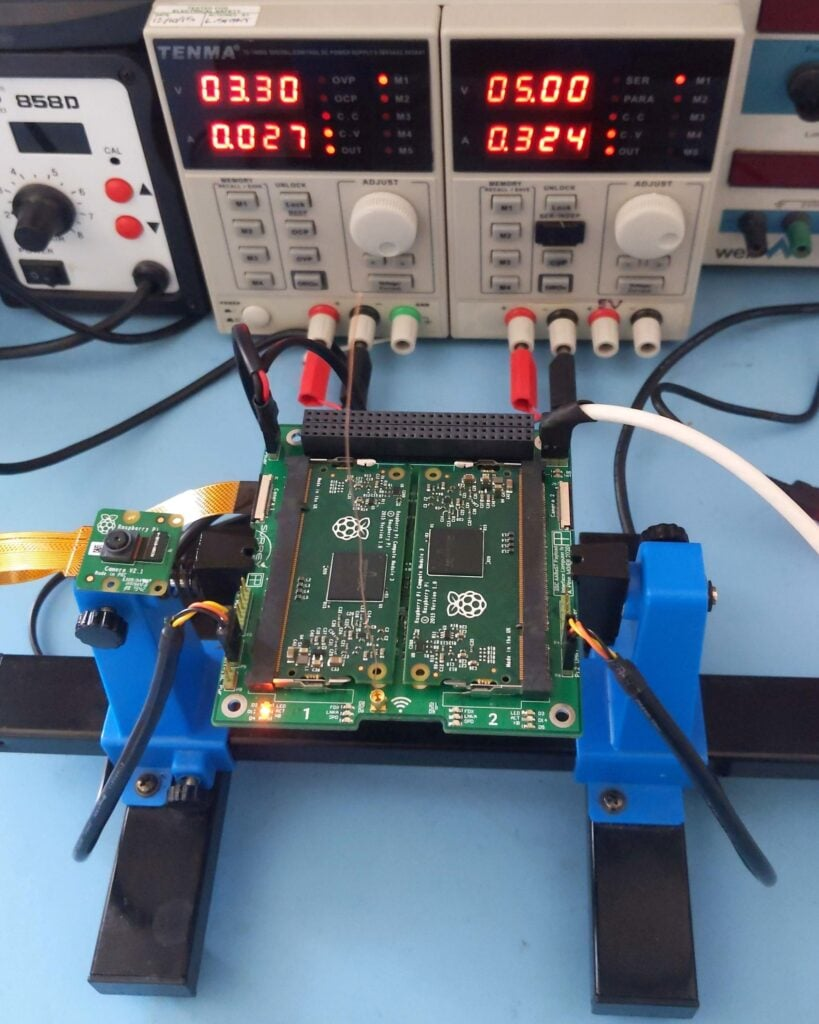
\includegraphics[width=0.8\textwidth]{../figures/cubesat_obc_rasp.jpeg}
        \end{center}
    \end{column}
\end{columns}

\vfill
\begin{block}{Definição}
    \textit{An embedded system is a computerized system that is purpose built for its application \cite{white_2024}.}
\end{block}
\end{frame}

\begin{frame}[fragile]
\frametitle{Revisão: Software embarcado}

\begin{columns}
    \begin{column}{0.5\textwidth}
        \textbf{Bare-metal:}
        \begin{enumerate}\small
            \item Controle direto e total do hardware;
            \item Ausência de overhead de sistema operacional;
            \item Máximo desempenho e otimização de recursos;
            \item Maior complexidade e tempo de desenvolvimento;
            \item Depuração mais desafiadora.
        \end{enumerate}
    \end{column}
    
    \begin{column}{0.5\textwidth}
        \textbf{SO:}
        \begin{enumerate}\small
            \item Camada de abstração de hardware;
            \item Gerenciamento de multitarefas e recursos;
            \item Facilita o desenvolvimento e aumenta a produtividade;
            \item Pequeno overhead de CPU/memória;
            \item Maior modularidade e manutenibilidade.
        \end{enumerate}
    \end{column}
\end{columns}

\end{frame}

\begin{frame}[fragile]
    \frametitle{Abordagens de implementação do software embarcado}

    \begin{center}
        % https://www.intel.com/content/www/us/en/docs/programmable/683211/current/bare-metal-overview.html
        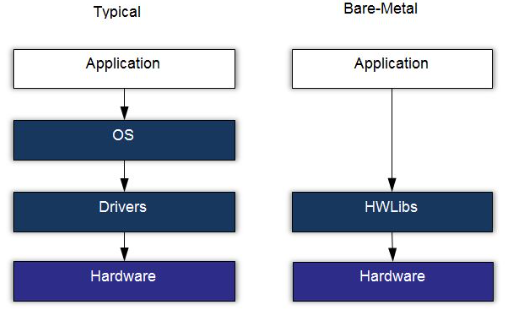
\includegraphics[width=0.6\textwidth]{../figures/bare_metal_vs_os.png}
    \end{center}

\end{frame}

\section{Introdução a SOs}

\begin{frame}[fragile]
    \frametitle{Sistema Operacional}

    \begin{columns}
        \begin{column}{0.55\textwidth}
            \begin{enumerate}\small
                \item Software essencial para FACILITAR o uso de sistemas computacionais;
                \item Permite a execução de múltiplos programas (aparentemente) simultaneamente;
                \item Gerencia os recursos de hardware do sistema computacional (e.g., CPU, memória, dispositivos de I/O);
                \item Portanto, pode ser visto sob duas perspectivas principais: máquina virtual e gerenciador de recursos.
            \end{enumerate}
        \end{column}
        
        \begin{column}{0.45\textwidth}
            \begin{center}
                % Diagrama ilustrativo da estrutura de um SO (e.g., camadas, kernel/user space)
                \includegraphics[width=0.85\textwidth]{example-image-a}
            \end{center}
        \end{column}
    \end{columns}
\end{frame}

\begin{frame}[fragile]
    \frametitle{SO como ``máquina virtual''}

    \begin{enumerate}\footnotesize
        \item A principal técnica utilizada é a ``virtualização'';
        \item Transforma recursos de hardware (e.g., CPU, memória) em formas virtuais mais gerais, poderosas e fáceis de usar;
        \item Abstrai detalhes complexos do hardware, provendo uma interface de mais alto nível;
        \item Oferece interfaces (APIs/chamadas de sistema) para que programas acessem funcionalidades e recursos;
        \item Contribui para a portabilidade das aplicações.
    \end{enumerate}

    \vfill
    \begin{center}
        % Diagrama de comunicação entre aplicação e hardware via SO, mostrando a abstração
        \includegraphics[width=0.5\textwidth]{example-image-a}
    \end{center}
\end{frame}

\begin{frame}[fragile]
    \frametitle{SO como gerenciador de recursos}

    \begin{columns}
        \begin{column}{0.55\textwidth}
            \begin{enumerate}\small
                \item Gerencia e aloca os recursos do sistema entre múltiplos programas:
                \begin{enumerate}\footnotesize
                    \item CPU (agendamento de processos/tarefas);
                    \item Memória (alocação e proteção);
                    \item Dispositivos de E/S (compartilhamento);
                \end{enumerate}
                \item Controla a execução de programas;
                \item Previne erros e o uso indevido de recursos;
                \item Otimiza o uso dos recursos com base em diversos objetivos.
            \end{enumerate}
        \end{column}
        
        \begin{column}{0.45\textwidth}
            \begin{center}
                % Diagrama ilustrando o gerenciamento de recursos pelo SO
                \includegraphics[width=0.85\textwidth]{example-image-a}
            \end{center}
        \end{column}
    \end{columns}
\end{frame}

\begin{frame}[fragile]
\frametitle{Kernel de um SO}

\begin{enumerate}\small
    \item \textbf{Kernel = Núcleo}
    \begin{enumerate}\footnotesize
        \item Parte central e fundamental de um programa/algoritmo
    \end{enumerate}
    
    \vfill
    \item \textbf{Kernel = Modo Kernel (Supervisor)}
    \begin{enumerate}\footnotesize
        \item Parte de um programa que executa em modo Kernel
        \item Modo Kernel -> Espaço/Modo de Execução
        \item Suporte do Processador a diferentes espaços ou níveis de execução (modo Kernel e modo usuário)
    \end{enumerate}
\end{enumerate}
\end{frame}

\begin{frame}[fragile]
\frametitle{Kernel de um SO}

\begin{enumerate}\small
    \item Núcleo do Sistema Operacional
    \item Provê o Gerenciamento do Sistema e Funcionalidades Básicas
    \item Executa em modo privilegiado (modo kernel)
    \item Controla acesso direto ao hardware
    \item Implementa serviços fundamentais:
    \begin{enumerate}\footnotesize
        \item Gerenciamento de memória
        \item Gerenciamento de processos
        \item Gerenciamento de dispositivos
        \item Comunicação entre processos
    \end{enumerate}
\end{enumerate}
\end{frame}

\begin{frame}[fragile]
\frametitle{Ambientes de Execução}

\begin{center}
    % Diagrama de camadas de abstração e anéis de privilégio
    \includegraphics[width=0.5\textwidth]{example-image-a}
\end{center}

\begin{enumerate}\small
    \item Diferentes níveis de acesso ao hardware
    \item Proteção contra operações indevidas
    \item Separação entre código privilegiado e não-privilegiado
\end{enumerate}
\end{frame}

\section{Tipos de Kernel}

\begin{frame}[fragile]
\frametitle{Abordagens de Design de Kernel}

\begin{enumerate}\small
    \item \textbf{Kernel Monolítico}
    \item \textbf{Microkernel}
    \begin{enumerate}\footnotesize
        \item Nanokernel
    \end{enumerate}
    \item \textbf{Kernel Híbrido}
    \item \textbf{Exokernel}
\end{enumerate}

\vfill
\begin{center}
    \textit{*Kernel Híbrido é tido como um termo controverso dentre a comunidade científica da área \cite{microkernel2007}.}
\end{center}
\end{frame}

\begin{frame}[fragile]
\frametitle{Kernel Monolítico}

\begin{columns}
    \begin{column}{0.55\textwidth}
        \begin{enumerate}\small
            \item Todo o sistema operacional executa em modo kernel
            \item Abordagem tradicional
            \item Exemplos:
            \begin{enumerate}\footnotesize
                \item Unix tradicional
                \item Linux
                \item FreeBSD
            \end{enumerate}
            \item Vantagens:
            \begin{enumerate}\footnotesize
                \item Desempenho
                \item Acesso direto ao hardware
            \end{enumerate}
            \item Desvantagens:
            \begin{enumerate}\footnotesize
                \item Menor segurança
                \item Falhas afetam todo o sistema
            \end{enumerate}
        \end{enumerate}
    \end{column}
    
    \begin{column}{0.45\textwidth}
        \begin{center}
            % Diagrama de kernel monolítico vs microkernel
            \includegraphics[width=\textwidth]{example-image-a}
        \end{center}
    \end{column}
\end{columns}
\end{frame}

\begin{frame}[fragile]
\frametitle{Microkernel}

\begin{columns}
    \begin{column}{0.55\textwidth}
        \begin{enumerate}\small
            \item Apenas funções essenciais no kernel
            \item Serviços executam como processos em modo usuário
            \item Comunicação via IPC (Comunicação Entre Processos)
            \item Exemplos:
            \begin{enumerate}\footnotesize
                \item MINIX
                \item QNX
                \item L4
            \end{enumerate}
            \item Vantagens:
            \begin{enumerate}\footnotesize
                \item Maior segurança
                \item Falhas isoladas
                \item Código mais modular
            \end{enumerate}
        \end{enumerate}
    \end{column}
    
    \begin{column}{0.45\textwidth}
        \begin{center}
            % Diagrama de arquitetura microkernel
            \includegraphics[width=\textwidth]{example-image-a}
        \end{center}
    \end{column}
\end{columns}
\end{frame}

\begin{frame}[fragile]
\frametitle{Conceitos e Objetivos do Microkernel}

\begin{enumerate}\small
    \item \textbf{Segurança}
    \begin{enumerate}\footnotesize
        \item Menor código possível executando em modo Kernel
        \item Menos tempo de execução do sistema em modo privilegiado
    \end{enumerate}
    
    \vfill
    \item \textbf{Separação de Serviços em Servidores}
    \begin{enumerate}\footnotesize
        \item Serviços executam como processos independentes
        \item Isolamento de falhas
    \end{enumerate}
    
    \vfill
    \item \textbf{Comunicação via IPC}
    \begin{enumerate}\footnotesize
        \item Baseada em troca de mensagens
        \item Mecanismo fundamental para operação do sistema
    \end{enumerate}
\end{enumerate}

\vfill
\begin{center}
    \textit{Abordagem proposta por Liedtke \cite{liedtke1995micro} para melhorar a segurança e modularidade}
\end{center}
\end{frame}

\begin{frame}[fragile]
\frametitle{Kernel Híbrido}

\begin{columns}
    \begin{column}{0.55\textwidth}
        \begin{enumerate}\small
            \item Combina características de kernel monolítico e microkernel
            \item Alguns serviços no espaço do kernel, outros como processos de usuário
            \item Exemplos:
            \begin{enumerate}\footnotesize
                \item Windows NT (Windows 10/11)
                \item macOS (XNU)
                \item DragonFly BSD
            \end{enumerate}
            \item Vantagens:
            \begin{enumerate}\footnotesize
                \item Equilíbrio entre desempenho e modularidade
                \item Flexibilidade de design
            \end{enumerate}
        \end{enumerate}
    \end{column}
    
    \begin{column}{0.45\textwidth}
        \begin{center}
            % Diagrama do kernel Windows NT
            \includegraphics[width=\textwidth]{example-image-a}
        \end{center}
    \end{column}
\end{columns}
\end{frame}

\begin{frame}[fragile]
\frametitle{Exokernel}

\begin{enumerate}\small
    \item Abordagem minimalista e radical
    \item Kernel fornece apenas proteção e multiplexação de recursos
    \item Bibliotecas em nível de usuário (LibOS) implementam abstrações tradicionais
    \item Desenvolvido no MIT nos anos 90 \cite{engler1995exokernel}
    \item Vantagens:
    \begin{enumerate}\footnotesize
        \item Máxima flexibilidade para aplicações
        \item Personalização de abstrações
        \item Potencial para alto desempenho
    \end{enumerate}
    \item Desvantagens:
    \begin{enumerate}\footnotesize
        \item Complexidade para desenvolvedores de aplicações
        \item Menor portabilidade
        \item Poucos sistemas em produção
    \end{enumerate}
\end{enumerate}
\end{frame}

\begin{frame}[fragile]
\frametitle{Comparação entre Tipos de Kernel}

\begin{center}
\resizebox{\textwidth}{!}{
\begin{tabular}{|l|c|c|c|c|}
\hline
\textbf{Característica} & \textbf{Monolítico} & \textbf{Microkernel} & \textbf{Híbrido} & \textbf{Exokernel} \\
\hline
Tamanho do kernel & Grande & Pequeno & Médio & Mínimo \\
\hline
Desempenho & Alto & Moderado & Alto/Moderado & Potencial alto \\
\hline
Modularidade & Baixa & Alta & Média & Alta \\
\hline
Segurança & Menor & Maior & Média & Variável \\
\hline
Complexidade & Alta & Média & Alta & Baixa (kernel) \\
 & & & & Alta (LibOS) \\
\hline
Exemplos & Linux, & MINIX, & Windows NT, & MIT Exokernel, \\
 & FreeBSD & QNX & macOS & Nemesis \\
\hline
\end{tabular}
}
\end{center}

\vfill
\begin{center}
    \textit{Cada tipo de kernel apresenta vantagens e desvantagens específicas \cite{tanenbaum2015modern}}
\end{center}
\end{frame}

\begin{frame}[fragile]
\frametitle{Interação de um Sistema com SO}

\begin{columns}
    \begin{column}{0.55\textwidth}
        \begin{enumerate}\small
            \item Comunicação entre aplicações e kernel:
            \begin{enumerate}\footnotesize
                \item Kernel Monolítico: System Calls e Sinais de Interrupções
                \item Microkernel: IPC, Kernel Calls e Sinais de Interrupções
            \end{enumerate}
            \item Diferenças fundamentais:
            \begin{enumerate}\footnotesize
                \item Monolítico: chamadas diretas ao kernel
                \item Microkernel: comunicação via mensagens entre processos
            \end{enumerate}
        \end{enumerate}
    \end{column}
    
    \begin{column}{0.45\textwidth}
        \begin{center}
            % Diagrama de comunicação do sistema
            \includegraphics[width=\textwidth]{example-image-a}
        \end{center}
    \end{column}
\end{columns}
\end{frame}

\begin{frame}[fragile]
\frametitle{Tendências Atuais em Design de Kernel}

\begin{enumerate}\small
    \item Sistemas operacionais modernos tendem a adotar abordagens híbridas
    \item Linux: kernel monolítico com módulos carregáveis
    \item Windows: kernel híbrido com componentes em modo kernel e modo usuário
    \item Sistemas embarcados: microkernels ganham popularidade pela segurança
    \item Virtualização e containers: novas demandas para design de kernel
    \item Sistemas de tempo real: foco em previsibilidade e determinismo
\end{enumerate}

\vfill
\begin{center}
    \textit{A escolha do tipo de kernel para sistemas embarcados depende dos requisitos específicos da aplicação \cite{stallings2018operating}}
\end{center}
\end{frame}

\begin{frame}{Resumo}
\begin{enumerate}\small
    \item Sistemas Embarcados podem ser implementados:
    \begin{enumerate}\footnotesize
        \item Bare Metal: programação direta no hardware
        \item Com Sistema Operacional: camada de abstração
    \end{enumerate}
    
    \vfill
    \item Sistemas Operacionais são camadas de software que gerenciam recursos de hardware
    
    \vfill
    \item Podem ser vistos como Máquinas Virtuais ou Gerenciadores de Recursos
    
    \vfill
    \item O Kernel é o núcleo do sistema operacional, executando em modo privilegiado
    
    \vfill
    \item Principais tipos de kernel:
    \begin{enumerate}\footnotesize
        \item Monolítico: todo o SO em modo kernel (Linux)
        \item Microkernel: mínimo em modo kernel, serviços em modo usuário (MINIX)
        \item Híbrido: combinação das abordagens anteriores (Windows NT)
        \item Exokernel: apenas proteção e multiplexação de recursos
    \end{enumerate}
\end{enumerate}
\end{frame}

\section{Referências}
\begin{frame}[t, allowframebreaks]
    \frametitle{References}
    \printbibliography
\end{frame}

\end{document}
